\section{Система Kerberos для локальной сети}\label{section-kerberos}
\selectlanguage{russian}

Система аутентификации и распределения ключей Kerberos основана на протоколе Нидхема~---~Шрёдера. Самые известные реализации протокола Kerberos включены в Microsoft Active Directory и ПО Kerberos с открытым кодом для Unix.

Протокол предназначен для решения задачи аутентификации и распределения ключей в рамках локальной сети, в которой есть группа пользователей, имеющих доступ к набору сервисов, для которых требуется обеспечить единую аутентификацию. Протокол Kerberos использует только симметричное шифрование. Секретный ключ используется для взаимной аутентификации.

Естественно, что в глобальной сети Интернет невозможно секретно создать и распределить пары секретных ключей, поэтому Kerberos построен для (виртуальной) локальной сети.

В протоколе используются 4 типа субъектов:

\begin{itemize}
    \item пользователи системы $C_i$;
    \item сервисы $S_i$, доступ к которым имеют пользователи;
    \item сервер аутентификации AS (\langen{Authentication Server}), который производит аутентификацию пользователей по паролям и/или смарт-картам только один раз и выдаёт секретные сеансовые ключи для дальнейшей аутентификации;
    \item сервер выдачи мандатов TGS (\langen{Ticket Granting Server}) для аутентификации доступа к запрашиваемым сервисам, аутентификация выполняется по сеансовым ключам\index{ключ!сеансовый}, выданным сервером AS.
\end{itemize}

Для работы протокола требуется заранее распределить следующие секретные симметричные ключи для взаимной аутентификации.
\begin{itemize}
    \item Ключи $K_{C_i}$ между пользователем $i$ и сервером AS. Как правило, ключом служит обычный пароль\index{пароль}, точнее, результат хэширования пароля. Может быть использована и смарт-карта.
    \item Ключ $K_{TGS}$ между серверами AS и TGS.
    \item Ключи $K_{S_i}$ между сервисами $S_i$ и сервером TGS.
\end{itemize}

\begin{figure}[!ht]
	\centering
	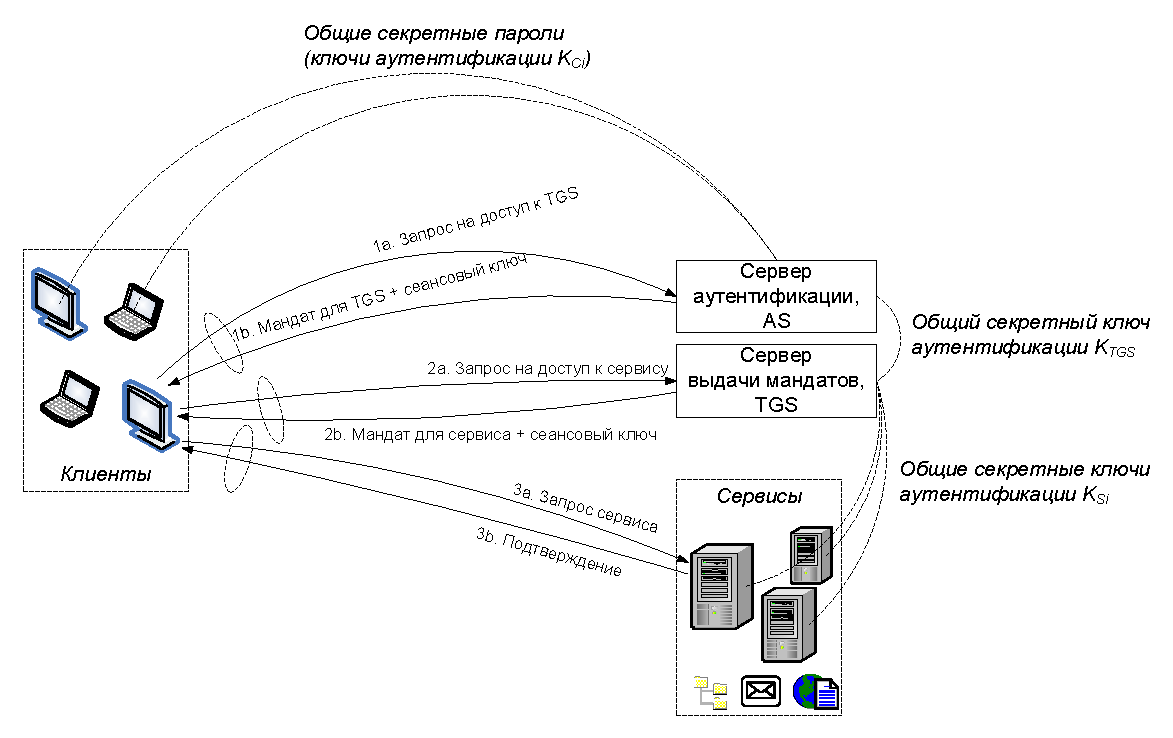
\includegraphics[width=\textwidth]{pic/kerberos}
	\caption{Схема аутентификации и распределения ключей Kerberos\label{fig:kerberos}}
\end{figure}

На рис.~\ref{fig:kerberos} представлена схема протокола, состоящая из 6-ти шагов.

Введём обозначения для протокола между пользователем $C$ с ключом $K_C$ и сервисом $S$ с ключом $K_S$:
\begin{itemize}
    \item $ID_C, ID_{TGS}, ID_S$ -- идентификаторы пользователя, сервера TGS и сервиса $S$ соответственно;
    \item $t_i, \tilde{t}_i$ -- запрашиваемые и выданные границы времени действия сеансовых ключей аутентификации;
    \item $ts_i$ -- метка текущего времени (\langen{timestamp});
    \item $N_i$ -- одноразовая метка (\langen{nonce})\index{одноразовая метка}, псевдослучайное число для защиты от атак воспроизведения сообщений;
    \item $K_{C,TGS}, K_{C,S}$ -- выданные сеансовые ключи аутентификации пользователя и сервера TGS, пользователя и сервиса $S$ соответственно;
    \item $T_{TGS} = E_{K_{TGS}}(K_{C,TGS} ~\|~ ID_C ~\|~ \tilde{t}_1)$ -- мандат (\langen{ticket}) для TGS, который пользователь расшифровать не может;
    \item $T_{S} = E_{K_S}(K_{C,S} ~\|~ ID_C ~\|~ \tilde{t}_2)$ -- мандат для сервиса $S$, который пользователь расшифровать не может;
    \item $K_1, K_2$ -- обмен информацией для генерирования общего секретного симметричного ключа дальнейшей коммуникации, например по протоколу Диффи~---~Хеллмана\index{протокол!Диффи~---~Хеллмана}.
\end{itemize}

Схема протокола следующая.
\begin{enumerate}
    \item Первичная аутентификация пользователя по паролю, получение сеансового ключа $K_{C,TGS}$ для дальнейшей аутентификации. Это действие выполняется один раз для каждого пользователя, чтобы уменьшить риск компрометации пароля.
        \begin{enumerate}
            \item $C \rightarrow AS: ~~ ID_C ~\|~ ID_{TGS} ~\|~ t_1 ~\|~ N_1$.
            \item $C \leftarrow AS: ~~ ID_C ~\|~ T_{TGS} ~\|~ E_{K_C}( K_{C,TGS} ~\|~ \tilde{t}_1 ~\|~ N_1 ~\|~ ID_{TGS})$.
        \end{enumerate}
    \item Аутентификация сеансовым ключом $K_{C,TGS}$ на сервере TGS для запроса доступа к сервису выполняется один раз для каждого сервиса. Получение другого сеансового ключа аутентификации $K_{C,S}$.
        \begin{enumerate}
            \item $C \rightarrow TGS: ~~ ID_S ~\|~ t_2 ~\|~ N_2 ~\|~ T_{TGS} ~\|~ E_{K_{C,TGS}}(ID_C ~\|~ ts_1)$.
            \item $C \leftarrow TGS: ~~ ID_C ~\|~ T_{S} ~\|~ E_{K_{C,TGS}}( K_{C,S} ~\|~ \tilde{t}_2 ~\|~ N_2 ~\|~ ID_S)$.
        \end{enumerate}
    \item Аутентификация сеансовым ключом $K_{C,S}$ на сервисе $S$ -- создание общего сеансового ключа дальнейшего взаимодействия.
        \begin{enumerate}
            \item $C \rightarrow S: ~~ T_{S} ~\|~ E_{K_{C,S}}(ID_C ~\|~ ts_2 ~\|~ K_1)$.
            \item $C \leftarrow S: ~~ E_{K_{C,S}}( ts_2 ~\|~ K_2)$.
        \end{enumerate}
\end{enumerate}

Аутентификация и проверка целостности достигаются сравнением идентификаторов, одноразовых меток и меток времени внутри зашифрованных сообщений после расшифрования с их действительными значениями.

Некоторым недостатком схемы является необходимость синхронизации часов между субъектами сети.
